% === above this line ===
% preamble
% begin document
% maketitle

\begin{abstract}
What is a developer's contribution to a repository? By only counting commits and number of lines changed, existing tools that analyze source code repositories fall short on showing the effective contributions made by each developer. When many commits are viewed as a group, the details are lost. Commit information can be misleading since lines of code give no indication of what was actually being worked on without careful examination of the changed code. Providing a semantic view of this information could provide deeper insights into how software projects evolve since changes to design and features are not clearly visible from line changes alone. We present TypeV: a method for visualizing Java source code repositories. Instead of counting line changes in a commit we extract detailed type information over time by using the differences between abstract syntax trees (ASTs). We are then able to track the additions and deletions of declarations and invocations for each type. Furthermore, we can track each author's type usage over time. Using TypeV, we examine specific cases in well-known repositories where our tool reveals interesting and useful information. We then compare type coverage information from the AST compared to file coverage to determine if unique information is provided by type information.
\end{abstract}

% no keywords

\IEEEpeerreviewmaketitle

\begin{figure*}[!t]
\centering
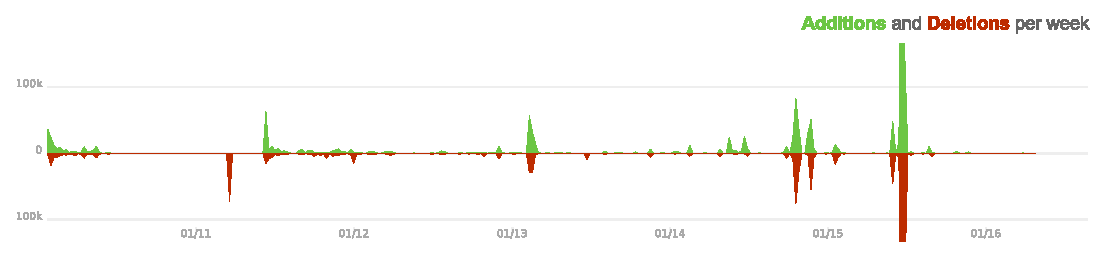
\includegraphics[width=\textwidth]{antlr4-code-freq}
\caption{GitHub graph showing code frequency. Note that the graph was truncated to better show the details, thus the changes that occur in mid 2015 are much larger than shown. The additions reach over 400k and the deletions are over 300k.}
\label{fig:GH_code_freq}
\end{figure*} 

\section{Introduction}

Source code is often represented as text in a source code file. This text is then parsed by a compiler or interpreter with the intent of eventually executing the instructions within the source code file. While programmers may type in individual characters, their intention is at a much higher level. Their intent is written in tokens that represent statements, identifiers and types that are used to solve their problems. Programmers solve problems in a way that is readable to other developers and executable by a computer. The programmer rarely operates at the character level, or even the line level, so why should our analyses of source code operate at granularities unfamiliar to developers?

The history and evolution of a software project is often tracked by version control systems, such as Git, in a programming language agnostic way. Updates to source code, documentation, and tests are recorded in the form of commits, which show the differences in lines between each subsequent revision of the software. Version control systems become vital for large projects since individual changes would be impossible to track manually. Large projects have thousands of individual changes made by many different developers. With more changes to peruse, it becomes more difficult to see how a project is evolving over time since there is so much information to look through. Most hosting services for Git repositories provide some basic tools for analyzing projects over time~\cite{github-graphs,bitbucket-graphs}; however, as we will show, these tools often lack the kind of detail to gather insightful analysis. While commits may store individual changes to lines of code, they represent the change in \emph{structure} of the software.  By visualizing lines changed, or files changed, the current state-of-the-art for software project visualization rarely capture the \emph{meaning} behind each commit; lines of code alone does not describe how a repository changed at a particular point in time. Thus, information regarding contributions from developers is often misleading since the number of commits and lines of code changed does not necessarily reflect meaningful changes to a repository~\cite{robles2014}.

Consider tools easily available to an open source software developer; for example GitHub graphs (see Figure~\ref{fig:GH_code_freq})~\cite{github-graphs}. Since GitHub tracks contributions based solely on number of commits and numbers of lines changes, data may be lacking, or even misleading. In the case of the Antlr4 project (Figure~\ref{fig:GH_code_freq}), the graph creates more questions than it answers. What happened at those big spikes of line changes in the graph? One of the spikes is so large, we had to truncate the graph to be able to show details of other changes. How did these large changes affect the code base? Who committed these large changes? Was it a team of contributors or one particularly prolific programmer? Plotting the number of lines changed may be misleading. A huge spike in additions may be caused by numerous reasons, such as the inclusion of automatically-generated documentation, the inclusion of an external library, or perhaps even a huge refactoring effort.

In this paper, we propose a method that analyses the changes in type usage and method invocations over time, as well as a tool to visualize this analysis, which we call TypeV. We claim that type usage offers more insight than line-based, file-based, and commit-based methods of visualization and analysis. Of the services we have surveyed, none of the tools visualize project evolution using granular type analysis per author via commit-by-commit abstract syntax tree differencing. For simplicity, we analyze only Java projects, as it allowed us to quickly develop and test our software. Since our approach described in this paper can be generally applied to any statically-typed language, we plan to extend it to other languages.

In Java, a type can be a primitive, provided by the language itself, or object references. Primitive types are those that are built into the language such as an \texttt{int} or \texttt{char}. Object references point to instances of classes. Classes are defined in the project itself or through an included library. The types in a project represent the functionality available for a developer to work with. Java's syntax encourages the creation of classes, thus we expect substantial Java projects to define many domain-specific types. Different parts of a program use different types and external dependencies. When writing or contributing to a project, the author's choice of which part of the program to edit will in turn affect what types they end up working with --- that is, it will affect the author's \emph{type coverage}.

Type information is useful for seeing what libraries and functions are being used.  For example, when a part of code becomes \emph{deprecated}, continuing its use may lead to design flaws or even security vulnerabilities. In Apache Nifi, an earlier version of the software used a compromised key-derivation functions; hence, this class was deprecated, but left in for compatibility with older versions of the software~\cite{nifi}. Viewing the type information of a change can show when usage of deprecated classes are added or removed from a project as well as how many remain over time. In a more general sense, we can see when types are being added or removed from the project as well as what types are heavily used throughout the project. Even better, we can see \emph{who} uses which types heavily.

Having tools for analyzing repositories based on type usage and method invocation would benefit many different parts of the software development process. Software management requires a high level understanding of the state of a repository and the changes being made which affect the functionality of the software. Tracking developer contributions in a less misleading way is also important for management since important contributions may be small and focused, but nevertheless, significant. Line difference (or simply, \emph{diff}) only provide meaningful information when they are analyzed by someone with familiarity with the source code being changed. Providing tools which bring more meaning to line differences would allow people less familiar with the code to understand changes being made. When large changes are made that cover many aspects of a project, it would also be useful to see how the change affects the software rather than a several thousand line diff.  Seeing how a project has changed over time is also vital for management since evaluating the state of completion of software can be very difficult.

In the following sections of the paper we will introduce a tool, TypeV, that we developed that visualizes changes to types used in a project over time. TypeV is able to extract type information from a repository by computing commit-by-commit abstract syntax tree differencing, which we describe in section~\ref{sec:methodology}. We seek to answer the following questions: \\ \\
\textbf{RQ1:} How can we extract type and method usage over time from repositories? \\ \\
\textbf{RQ2:} Does the type information give any interesting or useful insight into the project? \\ \\
\textbf{RQ3:} How does type coverage compare to file coverage?

\section{Related Work}

Analyzing source code is a popular research topic. Most of the focus is on how certain programming languages and features are used. However, there is no focus specifically on how types are used throughout a project.

Dyer \textit{et al.} \cite{Dyer:2014:MBA:2568225.2568295} mined AST nodes to study the use of new Java language features over time. They found that all new Java features do get used, but not nearly as often as they could have been. New features varied greatly in popularity and adoption rate. Developers would also modify old code to use new features as they were released. The authors also found the most popular features and how teams adopted new features. They did not check to see how much a developer used a feature but instead only checked to see if they used it at all.

Grechanik \textit{et al.} \cite{Grechanik:2010:EIL:1852786.1852801} examined the structure of Java programs mined from 2080 programs. This paper examined the breakdown of syntactic structures in open source repositories, however it does not consider per author statistics. 

Meyerovich and Rabkin \cite{Meyerovich:2013:EAP:2509136.2509515} surveyed developers and examined repositories to learn about language adoption and usage. Developers feel that certain language features are more important than others.

Parnin \textit{et al.} \cite{Parnin:2011:JGA:1985441.1985446} mined repositories to see how Java generics have been used in open source projects and found that generic usages were often introduced by a single developer in a project. Generics usage was also fairly narrow, with the primary use being collecting and traversing lists of objects.

Wagstrom \textit{et al.} \cite{Patrick:Wagstrom:2012} explored the roles that developers take in a networked, social development environments like GitHub. These role were defined as their level of contribution as well as the types of issues they dealt with. Developers will take on multiple roles in a project and will sometimes fulfill the same role across different projects.

L\"{a}mmel \textit{et al.} \cite{Lammel:2011:LAA:1982185.1982471} used ASTs to examine the usage of APIs in Java projects. They find what APIs are popular as well as if they are used in a framework like manner.

The aforementioned research is trying to learn how developers are using programming languages by looking at many repositories. This type of info can be extracted from individual repositories using our new tool. Type info may also provide additional information on how developers use languages.

Wu \textit{et al.} \cite{wu2004a} explore punctuated changes to software repositories with a tool that generates an Evolution Spectrograph. Each file has a representative row in the chart, with each cell in the row representing a section of time. This diagram would show changes to incoming and outgoing dependencies by darkening the cell where the change happened and lightening it over time if no changes were made.

In another paper, Wu \textit{et al.} \cite{wu2004} the Evolutionary Spectrogram is used but with greater control of granularity for files and software subsystems such as directory structure. Spectrograms are also used to display the cardinality of a developer's commits. The cardinality of a commit is the number of files or subsystems it affects in a system. All of the developers changes together show how many changes affect broad sections of the software.

Voinea \textit{et al.} \cite{voinea2006} visualizes CVS repositories using CVSgrab and adding their own enhancements to show changes to files over time. Files can be sorted by creation time, activity, or alphabetically and colour coded based on author, file size, file type or by search strings.

Kim \textit{et al.} \cite{Kim:2009:DRS:1555001.1555046} built a tool called Logical Structural Diff (LSdiff) which examines code changes and produces logical rules to represent them. Changes which do not match the rules are then pointed out to the developer. They also formed a focus group with software engineers who found that LSdiff complements existing tools well and showed promise for discovering inconsistent changes.

The service EasyBi \cite{EasyBi} provides additional visualizations for Git repositories for the purpose of business decisions. EasyBi works by taking the git log file and generating charts and graphs from it. It tries to solve the issue of summarizing many commits and has greater controls for granularity and authors but still operates on commits and line differences.

The Gitinspector project \cite{Gitinspector} is an open source tool for the statistical analysis of git repositories. It provides an advanced timeline view of changes per author and cumulative statistics but again relies upon the line differences to summarize the work of each author.

Wagstrom \textit{et al.} \cite{Patrick:Wagstrom:2012} explored the roles that developers take in a networked, social development environments like GitHub. These role were defined as their level of contribution as well as the types of issues they dealt with. Developers will take on multiple roles in a project and will sometimes fulfill the same role across different projects.

Lee \textit{et al.} \cite{lee2013} developed a tool for visualizing the branching structure of git repositories. This was used to analyze concurrent workflows in popular open source repositories.

The GitHub tools have the strength that they do not rely on what type of code is being committed. It does not matter what language or if errors exist in the commit, GitHub will simply spit out the number of line additions and deletions. The issue with this type of analysis is that it does not give a clear breakdown of is being changed only that changes have occurred.

\section{Methodology}
\label{sec:methodology}

\begin{figure}[!h]
\centering
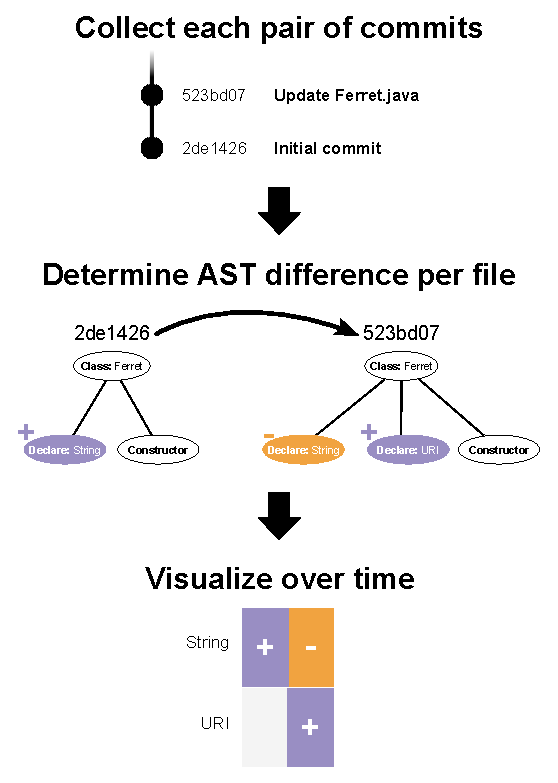
\includegraphics[width=\columnwidth]{context}
\caption{Shows the pipeline for TypeV. First we list the commits in chronological order. Then we perform AST diffs for each file. Finally, we display the information.}
\label{fig:context}
\end{figure}

Given a Git repository, we want to extract per-author type evolution over time. We accomplished this by computing the differences between abstract syntax trees of subsequent commits (Figure~\ref{fig:context}).

An \emph{abstract syntax tree} (AST) is a data structure derived from source code that breaks its syntactic constructs into a tree. Each node in the tree represents a syntactically valid chunk of code. This captures the structure of the code in an abstract and tractable manner. Converting raw source text to an AST is often one of the first steps performed by compilers. When a programmer makes a non-trivial change in code in a file, that difference will be reflected in the AST. This means that the AST of revisions in code repositories can be compared to see what structures a programmer is modifying.

The Java ASTs in our analysis were generated using Spoon~\cite{pawlak:hal-01169705}. Spoon is a tool for transforming and analyzing Java source code. It breaks code up into a meta-model including the AST itself. The model consists of three parts: structural elements, code elements and references to program elements. According to Spoon's authors: ''The structural part contains the declarations of the program elements, such as interface, class, variable, method, annotation, and enum declarations.  The code part contains the executable Java code, such as the one found in method bodies. The reference part models the references to program elements (for instance a reference to a type)''~\cite{pawlak:hal-01169705}. The Spoon model is convenient because it provides the infrastructure for performing AST differencing (described later) while retaining the code elements (such as type information) for analysis afterwards. Spoon also preserves all type and package (library) information, information vital to our semantic analysis.

To determine what has changed between two subsequent commits, we computed their \emph{AST difference}. An AST difference (or simply \emph{AST diff}) states which nodes were added and removed from a tree (step two in Figure~\ref{fig:context}). For this purpose, we used GumTree~\cite{falleri:hal-01054552}, an algorithm made to compute the difference between two ASTs generated by Spoon. For new files and deleted files we did not use GumTree; we were simply able to run Spoon on the files and treated everything as an addition or deletion respectively.

Once we generated ASTs, we were able to traverse through the trees to count the number of added or deleted \emph{declarations} and \emph{invocations} for a given type.

\begin{description}
\item [declaration] 
  Stating that use of a field or variable of a given type. For example declaration of a String type variable might look as follows:
  \\
  \begin{adjustwidth}{2.5em}{0pt}
  String myString; \\
  \end{adjustwidth}
\item [invocation] 
  A call site for a method that belongs to a type. For example an invocation of the trim method of a String type might look as follows:
  \\
  \begin{adjustwidth}{2.5em}{0pt}
  myString.trim(); \\
  \end{adjustwidth}
\end{description} 

An example of what our analysis tool might produce is as follows:

\begin{verbatim}
#DECLARE | INSERT | java.net.URI | 2
#DECLARE | DELETE | java.lang.String | 2
\end{verbatim}

This states that two declarations of type \texttt{java.net.URI} were added, and two declarations of type \texttt{java.lang.String} were deleted. Note the fully qualified type names. The source text may not literally have the characters \texttt{java.net.URI}, but Spoon was able to infer from the import statements in the Java source text that references to ''URI'' resolve to the fully-qualified type name \texttt{java.net.URI}. Thus, TypeV is able to keep track of the actual class being used and is not confused when two classes in separate packages have the same name.

\begin{figure}[!h]
\centering
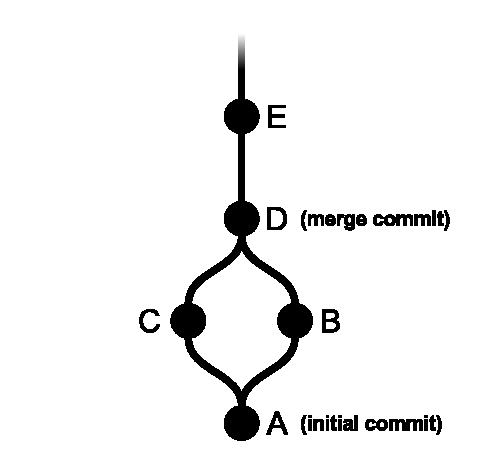
\includegraphics[height=2.5in]{commits_view}
\caption{Commits increase in time from bottom up. Therefore, ASTs from B and C are diff'd against ASTs in A. ASTs from E are diff'd against D. Since D is a merge commit, its changes are ignored as they are recorded in C and B.}
\label{fig:commits}
\end{figure}

In order to gather all the changes for a given repository over time, we generated ASTs for each commit and compared the difference. We did this by running \texttt{git log} over the Git repository and listing all the commit IDs in chronological order (Figure~\ref{fig:commits}). Each commit and its parent were then compared using AST differencing as described above. There are a few edge cases; however, if a commit has no parent, then every declaration or invocation in the commit was treated as an addition. Since we compared each commit to its parent, as reported by Git, we were able to account for any branching that happened outside the primary branch of the repository (usually named \texttt{master}). If a commit has more than one parent, this indicates a merge commit in Git. Merge commits contain the changes made in each parent commit combined. Therefore, we ignored merge commits since all changes in the merge should already have been accounted for in previous commits. Thus, any branch that has been merged into the primary branch would have been analyzed and included by TypeV.

\section{TypeV: The Visualization Tool}

\begin{figure*}[!t]
\centering
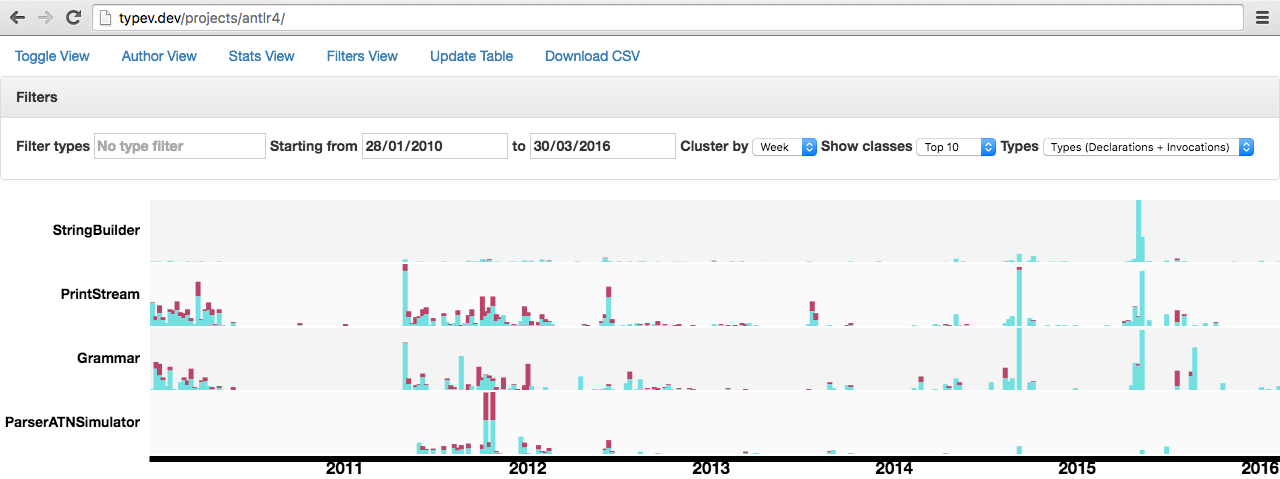
\includegraphics[width=\textwidth]{Screenshot_antlr4}
\caption{Screenshot showing the main view for TypeV. The data being displayed is from the antlr4 repository.}
\label{fig:main-view}
\end{figure*}

The data would be difficult to analyze if displayed as its raw text form; instead, we created an HTML5 web visualization application which is intended for developers, project managers, and researchers to use (Figure~\ref{fig:main-view}). The source code for TypeV is available online on GitHub,\footnote{\url{https://github.com/mdfeist/TypeV}}.

TypeV provide a variety of views to help organize the data and provide different levels of detail. The main view displays a series of stacked bar graphs which show changes to types over a period of time in a project (Figure~\ref{fig:main-view}). The blue and orange portions account for the number of additions and deletions in a similar fashion to GitHub’s code frequency graph (Figure~\ref{fig:GH_code_freq}). The height of each bar shows the number of changes to a type. The width of each bar represents a set time period and can be changed to an hour, day, week, or month. A bar which fills the row vertically is the period with the largest number of changes to that type out of the visible time periods. The other bars in the row are proportional to that maximum number.  The bar height is calculated by multiplying the maximum bar height by the number of changes during that time period divided by the maximum number of changes attested for this type. The rows are sorted so that the graph for the most used types appear the top and are in descending order.

When a user mouses over a specific bar in the graph they are given information for the type and time period at that location. The information includes the fully-qualified name of the type, the number of commits, the number of authors, the number of additions, the number of deletions, and the start and end date of that time period. If the user clicks on the bar, they are given more detailed statistics which list the authors who made the commits and each commit message.

One issue with analyzing individual authors is that authors can commit from a variety of different computers which can have different emails and usernames attached to the Git configuration. This may result in one author appearing as several different users in the \texttt{git log}. There is no perfect way to deal with this problem; however, we allow the user of our software to select and view multiple users at a time, thus allowing the user to view changes from an individual or group of developers.

To allow for a more detailed analysis of a specific component of the repository we added some basic filtering tools. First a user can filter by type name. Second the user can view changes that fall within a specific start and end date. Third the user can specify the time span represented by each bar: hour, day, week, or month. Finally, the user can choose to see only declarations of types, types used in declarations and invocations, or only invocations.

\section{Evaluation}

\begin{table}[!t]
\renewcommand{\arraystretch}{1.3}
\caption{Comparison of Type Coverage and File Coverage in Projects}
\label{tab:summary}
\centering
\begin{tabular}{c|ccc}
\hline
\bfseries Project & \bfseries Wilcoxon& \bfseries Pearson (linear) & \bfseries Spearman (rank) \\
& $p$-value & Correlation & Correlation \\
\hline
antlr4 & $p\ll0.01$ & 0.943 & 0.907\\
bookkeeper & $0.313$ & 0.984 & 0.972\\
curator & $0.007$ & 0.975 & 0.980\\
tika & $0.653$ & 0.955 & 0.998\\
\hline
\end{tabular}
\end{table}

\begin{figure}[!h]
\centering
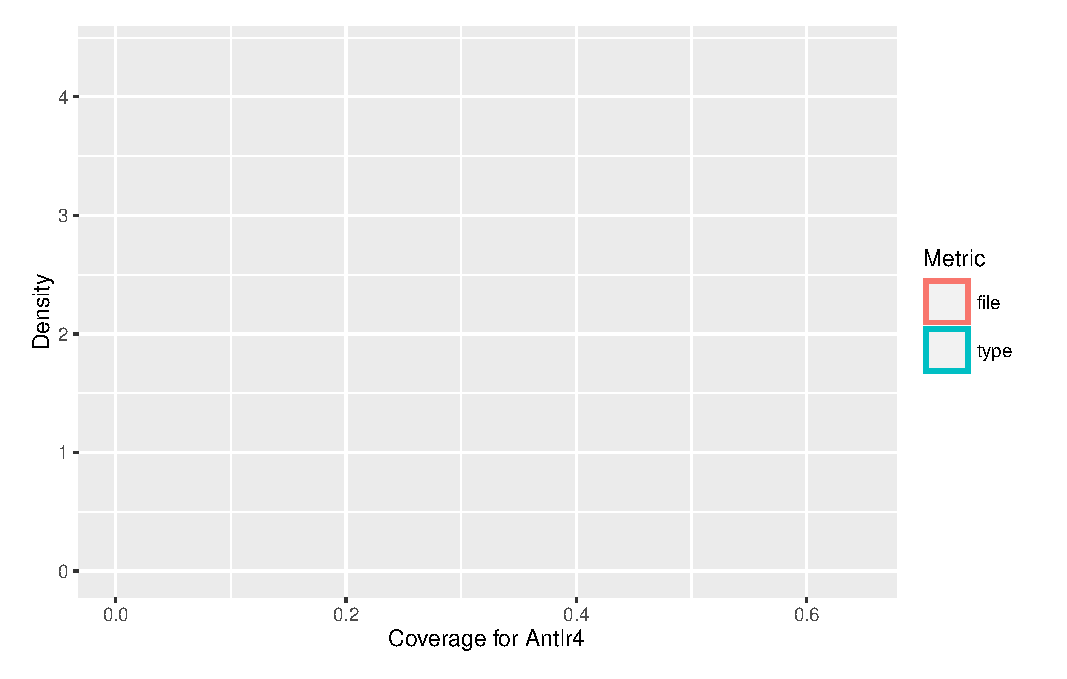
\includegraphics[width=\columnwidth]{antlr-density}
\caption{}
\end{figure}

\begin{figure}[!h]
\centering
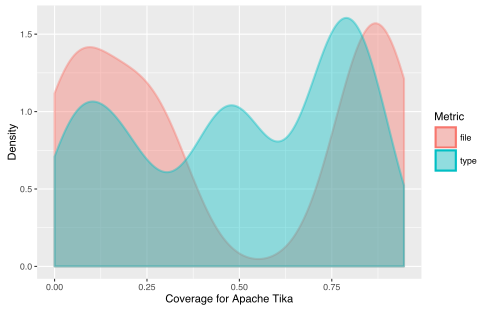
\includegraphics[width=\columnwidth]{tika-density}
\caption{}
\end{figure}

The information regarding which types are used in each change is unique to the AST diff method, so it will be useful to see how changes affect the types in a project rather than just the files involved in a diff. We define type coverage as the number of types that have been touched out of the total number of types during either a certain time period or the entire project. File coverage is the same measurement, but using the number of source files instead. To determine if type coverage gives different information than file coverage, we analyzed four popular Java projects: Antlr, Apache Bookkeeper, Apache Curator and Apache Tika. We counted the file coverage and type coverage on a commit-by-commit basis. That is, each datum represents a commit with three dimensions: file coverage and type coverage, and its commit date. Data is sorted in ascending order of commit date. Table~\ref{tab:summary} lists a summary of the data provided. In general, all measures are strongly correlated, both for Pearson (linear) correlation, and Spearman (rank) correlation. As type coverage and file coverage are both cumulative measures, positive correlation is expected. However, even when the distributions are significantly different (as with Antlr and Curator), the correlation is still strongly positive, but not 100\%. This means that when the coverage for types and files of a commit increase, the relationship is not necessarily 1-to-1. This is remarkable in a language like Java, a classes and files are generally in a 1-to-1 relationship.We conclude from this that type coverage yields related, yet different information than file coverage alone.

\section{Case Study}

In the following sections we present case studies demonstrating the extra insight that the TypeV method makes available.

\subsection{antlr4}

\begin{figure}[!ht]
\centering
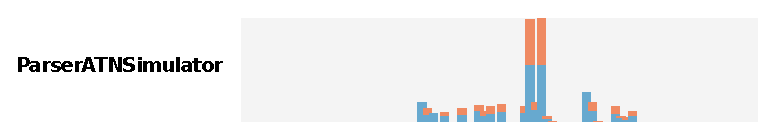
\includegraphics[width=\columnwidth]{ParserATNSimulator}
\caption{Snapshot of TypeV showing changes to ParserATNSimulator in antlr4. Date ranges from approximately the begining of 2011 to the end of April, 2012.}
\label{fig:parser1}
\end{figure}

\begin{figure}[!ht]
\centering
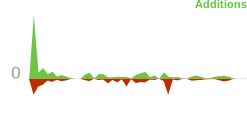
\includegraphics[width=\columnwidth]{Antlr4-GH-Lines-ParserATNSimulator}
\caption{GitHub's line difference graph showing changes to antlr4. The time spans approximately the same length as Figure~\ref{fig:parser1}.}
\label{fig:parser2}
\end{figure}

We chose Antlr4 because it is a substantial Java project with a commit history spanning several years. We can also see distinct changes throughout its history.

For example, in December of 2011 we can see that the ParserATNSimulator class has a large amount of additions and deletions in roughly equal proportion (Figure~\ref{fig:parser1}). This suggests that ParserATNSimulator is not being removed from the project but instead there is some refactoring being done. If we take a closer look at the commit messages we can see that they mention refactoring and reorganization of code. Zooming in on that date,  shows that during that month they were finishing work on a new version of ParserATNSimulator.

If we tried to do the same analysis with the GitHub tools it would be significantly more difficult to achieve the conclusion achieved using TypeV (Figure~\ref{fig:parser2}). First if we only look at line changes this change to ParserATNSimulator is overwhelmed by other changes and hardly shows up on the GitHub tools. If we did notice an increase in activity we would not know what types were being worked on. Finally, we could not quickly look at the commit messages for that specific time and type if we used the GitHub tools.

Using TypeV we can can see that at certain times there were major changes across all types. This shows us when major changes to the code were being done versus code maintenance. 

\subsection{Apache Bookkeeper}

\begin{figure}[!ht]
\centering

\includegraphics[width=\columnwidth]{bookkeeper_dep}
\caption{Shows deprecated invocation getLedgerManagerType() and replacement invocation getLedgerManagerFactoryClass() for Apache Bookkeeper.}
\label{fig:bookkeeper-depr}
\end{figure}

For deprecation analysis, we chose Apache Bookkeeper. As an Apache Foundation project it is a well-curated example of an open source software project. It also demonstrates an instance of deprecated methods. 

Apache Bookkeeper deprecated the method AbstractConfiguration.getLedgerManagerType() in release 4.2.0\footnote{\url{https://bookkeeper.apache.org/docs/r4.2.0/apidocs/deprecated-list.html}} and replaced it with AbstractConfiguration.getLedgerManagerFactoryClass(). If we look at getLedgerManagerType() we can see at the time of the start of the deprecation all instances were removed and getLedgerManagerFactoryClass() was added (Figure~\ref{fig:bookkeeper-depr}). After the deprecation, we see no more changes to getLedgerManagerType() and only some additions of getLedgerManagerFactoryClass().


\section{Discussion}

When managing group projects in an introductory software engineering course, it is very important to be able to see the contributions that students are making to the group repository to judge learning, progress and collaboration. When supervising 4-5 groups of students, it becomes unfeasible to look through all of the commits of each student. Students may take the wrong approach in a certain piece of code which becomes ingrained in the project and very difficult to change. Many groups have problems with group members who do not complete their assigned work or make contributions which end up being meaningless. Issues like this can be difficult to detect and prevent. As a manager, having a tool like TypeV allows one to quickly summarize the work done by each group member, organized by the types they have been working on. This can show when intervention or guidance is required, without the large time commitment of looking through commits.

The purpose of deprecated software features is to give developers time to change projects to follow a new or better standard without breaking the code. Deprecated features can be marked for removal from a project or have some flaw that would make a different feature the better option. Given the time at which a feature was deprecated, seeing the progress of replacement has some important implications. In the case of a security flaw, that time could indicated times at which systems or users were vulnerable. If a feature is marked for removal, a project using a deprecated type has a limited amount of time to make the changes. Removing all instances of deprecated features could also mean a project can be upgraded to use new tools or features that were not possible while the deprecated features were present.  Here we show examples where deprecated classes were removed.

Bug triaging for large open source projects is a very time consuming task, with hundreds  of bugs being reported daily. Each bug must be processed and assigned to a developer that has the experience required to fix the bug. In order to be effective, the triager has to have knowledge of what each developer has worked on as well as the parts of the code may be affected by the bugs. Being able to directly see what types a developer has worked with over time is important information for triaging. If the type causing the bug is known, the developers which have recently used that type can be assigned the bug. The commit messages for the affected types are also visible, providing greater context about how the type has been used. The developer who is assigned the bug can also use type information to locate other affected pieces of code and know which developers have been using the affected types.

\subsection{Threats to Validity}

Some commands in git present a problem gathering the statistics. Authors can pull other projects into the repository and these additions will count towards the author's changes. These will show up as massive changes by a single author with many types that they did not actually create. Changes of this size are visible in the graph and can be found by inspecting the commit messages.

We only look at the master branch of a repository and ignore other branches; therefore, we might miss some of the work done by an author in another branch. Going through all of the branches in a repository would take a very long time and contain a large amount of duplicate data. Being able to choose which branch to analyze is something that can be added.

We ignore the merge commits so we do not double count changes; however, if there is a merge conflict and the developer makes changes then these changes will not appear in TypeV. We make the assumptions that if this case happens then the changes are minor.

\subsection{Future work}

Currently, we treat every instance of a generic type as a different type. For example, considered the \texttt{List<T>} generic class in Java. If a user declares a List of Strings and later declares a List of Integers these will appear as two different types in TypeV. However, if they declare multiple instances of a List of Strings then these instances will count toward the same type. In the future, we want to work on a better way to track and represent generic types.

Currently we are only looking at declaration of types and invocation of methods; it would be useful to also view what classes changes are being made to. Enabling this ability would also enable analysis of self-invocations.

The methodology used in TypeV is only well-defined for statically-typed languages such as Haskell or Java; it is not well defined for dynamically-typed languages such as Erlang or JavaScript. However, type annotation systems such as TypEr for Erlang~\cite{typer} or statically-typed language dialects such as TypeScript for JavaScript may prove to be sufficient to enable type analysis as we have demonstrated for Java.

\section{Conclusion}

In this paper, we introduced TypeV, a source code repository analysis and visualization tool. Its use of commit-by-commit abstract syntax tree differencing enable for more insightful visualization than tools that merely use commit counts, line counts, and file changes. We answered our research questions as thus:

RQ1: Using abstract syntax trees, we can determine the types affected by each commits in a repository. Type information is not directly available through regular line diffs recorded by Git.

RQ2: The evolution of a project and developer activity can be seen through the changes to types in a project. Significant events can be observed with greater understanding by seeing the changes to types in addition to the existing commit information.

RQ3: Type coverage and file coverage are found to be highly correlated but do not always have the same distribution or a one to one ratio as might be expected in Java.


% === Below this line ===
% bibliography
% end document
